\documentclass[conference]{IEEEtran}
\IEEEoverridecommandlockouts
% The preceding line is only needed to identify funding in the first footnote. If that is unneeded, please comment it out.
\usepackage{cite}
\usepackage{amsmath,amssymb,amsfonts}
\usepackage{algorithmic}
\usepackage{graphicx}
\usepackage{textcomp}
\usepackage{xcolor}
\def\BibTeX{{\rm B\kern-.05em{\sc i\kern-.025em b}\kern-.08em
    T\kern-.1667em\lower.7ex\hbox{E}\kern-.125emX}}
\begin{document}

\title{Keypad Entry System\\
Group 4: Gamechangers
}

\author{\IEEEauthorblockN{1\textsuperscript{st} Ben Henaghan}
\and
\IEEEauthorblockN{2\textsuperscript{nd} Scott Wang}
\and
\IEEEauthorblockN{3\textsuperscript{rd} Austine Yapp}
\and
\IEEEauthorblockN{4\textsuperscript{th} Mike Yue}
}

\maketitle

\begin{abstract}
This document is a model and instructions for \LaTeX.
This and the IEEEtran.cls file define the components of your paper [title, text, heads, etc.]. *CRITICAL: Do Not Use Symbols, Special Characters, Footnotes, 
or Math in Paper Title or Abstract.
\end{abstract}

\begin{IEEEkeywords}
component, formatting, style, styling, insert
\end{IEEEkeywords}

\section{Introduction}
Digital door locks are becoming more and more common, and as they become more common, the vulnerabilities they suffer from become more and more dangerous. While digital locks are more convenient by offering a keyless entry and exit, they are susceptible to a slew of different attacks, all intended to derive the static PIN that unlocks the digital lock.

\subsection{Problems with traditional keypad entry systems}

Assuming a 4 digit access code, simple wear and tear on the keypad means that the attacker only needs to try 4! (24) combinations at most to bruteforce the PIN, cutting down the original keyspace by almost 98\% (Figure 1).

\begin{figure}[h!]
  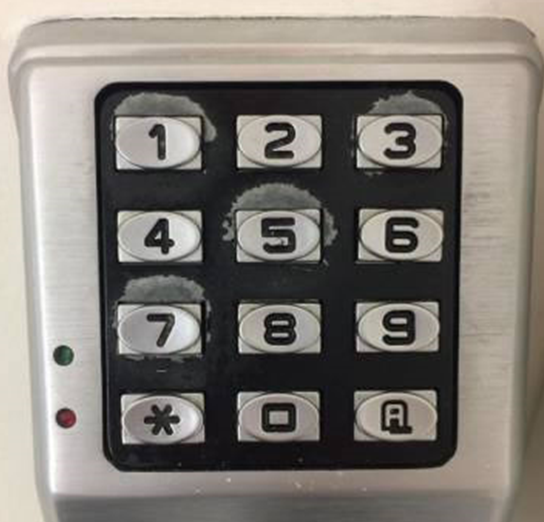
\includegraphics[width=\linewidth]{worn_lock.png}
  \caption{Worn keypad exposes digits of PIN}
  \label{fig:wornlock}
\end{figure}

More active attacks include shoulder surfing or installing inconspicuous pinhole cameras over the lock, revealing to the attacker exactly what the combination is if the victim is unaware of the attack. 

Clearly, this is a security problem, one that hinges on the assumption of a static PIN code. Therefore, we seek to address this problem by dynamically and randomly generating temporary access codes for the user on demand, rather than having the lock accept a preset access code. In other words, our system will have the digital lock, by default, reject every input as invalid. Only when users request a new code through our mobile app will the lock accept the newly generated code.

\subsection{Importance of Problem}
It can be hard to quantify or estimate the value of goods protected by electronic keypad locks. We postulate that if the location is important enough to secure with an electronic keypad lock, then the user does not want the location compromised, and thus security is important to the user. 

	However, these electronic keypads allow users to choose their own static access codes, and humans are wildly unsuited to coming up with random PIN codes. Analysis done on leaked 4 digit PINs from breaches or leaks found that 1234 accounted 11\% of the 3.4 million leaked codes, and the top 20 most common PINs accounted for 26.83\% of the entire 3.4 million PINS \cite{b1}.
	
	Clearly, users cannot be trusted to come up with secure random access codes, and thus cannot effectively protect themselves, which is an important problem that our design seeks to address.


\subsection{Proposed Solution}

\subsection{Contributions}
The work on the prototype was split naturally over the three components --- The mobile application, server application and code which would run on the actual lock hardware.
It was deemed that the android (mobile) application would form the largest amount of work, so that was split between Ben Henaghan and Scott Wang who both had some experience writing mobile applications.
Mike Yue developed the server code and Austine Yapp produced the software for the lock hardware.

\section{Related Work}

\section{Adversary Model}
To truly explore the strengths and limits of our system, we must put ourselves in the shoes of the adversary, and reason about the objective and capabilities of such an adversary.
\subsection{Objective of Adversary}
The adversary has the primary objective of gaining authorized access to the secured location by entering through the door secured by a digital lock. Forced entries, whether through the secured door or other entrances, are unauthorized accesses and thus outside the scope of this adversary. To achieve this, the adversary seeks the valid PIN code to the digital lock. We assume this adversary is an opportunistic burglar, who does not care about which location they break into and will target the easiest location.
\subsection{Capabalities}
	This adversary can install any arbitrary system on or around the digital lock that will not be noticed by the regular user, including tools such as keyloggers and pinhole cameras. Furthermore, through sleight of hand or other means, the adversary can steal the phone of the user, which has the mobile application that requests new codes installed on it. Furthermore, through social engineering, shoulder surfing, or just bruteforce, the adversary is able to unlock the user’s phone and launch the mobile application.


\section{System Design}

\subsection{Principles of Secure System Design}
Our design satisfies a number of secure system design principles.
\begin{enumerate}
\item{Open Design: The security of our system is not based upon the secrecy of our design or implementation. Even if attackers gained access to the complete source code of our project, they would be unable to predict the next PIN code generated for any arbitrary lock from the server, and unable to gain access to any mobile application accounts to generate new PIN codes.}
\item{
Economy of Mechanism: The method with which we generated new PIN codes, as well as the method of communication between server/lock/application have been chosen to be as simple and small as possible.
}
\item{
Complete Mediation: Every single request to the server requests authorization, and every new PIN code request on the application requires biometric confirmation before it is carried out.
}
\item{
Least Privilege: Basic users can only generate new PIN codes or fetch the current existing code, and cannot add new users to be associated with their locks.
}
\item{
Psychological Acceptability: The system was designed to be as seamless as possible for the user. While there will obviously be more friction than if this system did not exist, we attempted to minimize the impact on users.
}
\item{
Separation Privilege: Users can only generate new pin codes if they are logged in AND have access to the lock they are trying to generate the pin code for. Thus, new pin codes are granted based on more than one condition.
}
\item{
Fail-Safe Defaults: By default, locks do not have any valid access codes. By default, users do not have access to any locks until the lock administrator user grants the user access to the lock. By default, the server does not accept any incoming requests unless they are logged in and authenticated.
}
\end{enumerate}


\section{System Prototype}
\subsection{Server}
The server acts as the central hub, accepting communications from both the digital lock and mobile application. All communications are done via HTTPS, making eavesdropping impossible. Furthermore, any requests to generate new PIN codes or access available locks must be authenticated. To this end, the server requires the mobile application to first log in and provide valid credentials, after which the server will provide a token which must be provided with every subsequent request for authentication. If a valid request is made to generate a new access code, the server uses true random number generatino to generate a new code, tag it with the requested expiry time, and returns the code to the client.

The digital lock will only send its own serial number and the code it received to the server. This is the only action on the server that does not require authentication. Upon receiving a valid code, the server immediately marks the code as invalid, rendering any subsequent requests with the same code invalid as well. The only viable attack against this would be to constantly bombard the server with every 4 digit PIN between 0000 and 9999, thus denying everyone access. This could be easily mitigated by limiting the number of requests the server takes from the same IP address. Furthermore, denial of access is against the interest of our adversary model, who wishes to enter the location.


\section{Evaluation}
\newpage
ajaj
\newpage
\section{Discussion}
In this section, we will discuss the advantages and benfits of our system prototype and its broader design.
We will then examine its limitations and disadvantages.
Finally, we will consider the findings of our project overall, with these aforementioned `pros' and `cons' in mind.

Our prototype system is complete enough for us to draw useful conclusions about a similar potential product but is by no means a complete system in of itself.
The simple design allowed the development team to produce an MVP (Minimum Viable Product) and then iterate on this initial product to build our prototype system.
Fundamentally, our system only comprises a subset of the hardware needed for an electronic door lock, namely the authentication and control electronics.
Many non-core processes have been omitted from our prototype, namely a secure lock enrollment method and a full logging system.
Although our prototype was missing these features, we were still able to collect significant data about the usability of this kind of system, which could easily be incorporated into a future commercial security device.

\subsection{Advantages}
User testing showed that users appreciated the clear security benefits of our system but did find it to be a slight inconvenience.
The trade-off of security and convenience is a core problem when designing security products for use by the general public; users will be hesitant to opt-in to enhanced security measures if they deem it to be a significant inconvenience.
It has been shown that almost two-thirds of users will select the least secure and most convenienent security option if given the choice \cite{bben1}.
Our system seeked to strike a good balance between the extra security benefits of TOTP codes and the convenience of a numeric keypad lock.

All types of shoulder-surfing and replay attacks are completely defeated by our device, meaning that there aren't many possible `subtle' (ie non-destructive) attacks against our system.
However, it is worth noting that the Wi-Fi connected electronics, mobile application and server are all attack surfaces not present in standard keypad-operated access control systems.
Overall risk incurred by the device is therefore reduced, as the vulnerability value is significantly decreased.

Given our adversay model, our device successfully resists most known capabilities, such as replay attacks with pinhole cameras.
The adversary model does also assume that they would be able to gain access to the user's phone using a social engineering attack, and given access to the phone it is possible that the adverary would be able to comprimise the system.
This is because if the threat agent is able to unlock the phone, they should be able to enrol their own biometrics and therefore activate the code generation in the android application.
The risk of access in this way is mitigated in a few different ways.
Enrolling a fingerprint with android  and then generating an unlock code would typically takes upwards of a minute, which would likely arrouse the suspiscion of the owner.
The impact of this kind of attack could be further reduced if guidance was added to the android application telling users to be aware of such social engineering attacks and not to share their phone wiht strangers without being aware of what they're doing.
The other mitigation of this kind of attack relies on the expiry time of the single-use code, as the adversary would have to get to the door lock in time to use the comprimised code --- which is likely take a significant amount of time due phsycial distance.
A sophisticated attack could have another adversary located closer to the door, but this level of organization is uncharacteristic for an oppourtunistic threat agent.

\subsection{Limitations}
As mentioned before, the phsycial security of our prototype device was out of scope for this project, but would be an important part of the design if we wanted to bring a product like this to market.
Our prototype, however, did suffer from a few limitations which impeded both security and usability.

An auto-login feature would greatly improve user effiency, and would not impair security significantly, as biometrics would still be needed to generate a code.
This enhancement to the mobile application could easily half the time needed to generate a code in the app, as currently the app will force a user to log in manually if it has not been opened recently (if the activity has not yet been started or has been killed by android).
Currently, this limitation significantly impairs the user experience of using our entire system, as typing a username and password is not only a time consuming acitivity, but a fairly difficult and precise process.
Most users would have to stand still in order to do this, which is frustrating for a potential user.
With an auto-login feature no precise actions are required, meaning a user could generate a code as they walk up to the door and would only have to stop to type in the code --- the same as a traditional keypad lock.

Somewhat counter-intuitively, it would increase the overall security of the system to remove the ability of users to manually set the expiry time of codes.
The current behavior limits the effectiveness of the TOTP codes and encourages users to generate codes ahead of time, making the system much less secure.
This would force codes to always expire after a certain, short, amount of time (eg two minutes); which would force users to only generate codes when they intent to use them immediately.
Another benefit of this change would be that the speed of generating a code would improve, as it would be another step that the user would not have to do.

Another significant limitation of our design is that a planned `failure mode' was not integrated. This is where the lock would accept a more secure (eight digits) long-term code to unlock if the user was to not have access to their phone.
This was not implemtned into our prototype due to the additional development effort that would be needed
It does, also, pose a signficant security issue --- as it subverts a signficant amount of the security design in the core product.
We demed that it would be neccesairy in a commercial product but did not resolve the challenges associated with designing such a protocol, essentiall making it easy for the legitimate users while keeping the lock secure.
This would be a great avenue for future research.

\subsection{Overall Findings}
Overall, we found that security was significantly increased by using our system in place of a traditional keypad lock, when using our defined adversary model.
However it is, of course, more inconvenient to use our system over a traditional keypad-based access control system. 

We believe that the compromise is likely to be accepted by the majority of security-conscious consumers, as well as many large corporations currently utilizing keypad door locks.
Corporations pose signficant potential customers for this kind of system, as the value of assets protected by access control systems can be massive, and the traceability offered by a system such as ours would be very useful when many different people might need access at different times.

\section{Conclusion}

% \begin{table}[htbp]
% \caption{Table Type Styles}
% \begin{center}
% \begin{tabular}{|c|c|c|c|}
% \hline
% \textbf{Table}&\multicolumn{3}{|c|}{\textbf{Table Column Head}} \\
% \cline{2-4} 
% \textbf{Head} & \textbf{\textit{Table column subhead}}& \textbf{\textit{Subhead}}& \textbf{\textit{Subhead}} \\
% \hline
% copy& More table copy$^{\mathrm{a}}$& &  \\
% \hline
% \multicolumn{4}{l}{$^{\mathrm{a}}$Sample of a Table footnote.}
% \end{tabular}
% \label{tab1}
% \end{center}
% \end{table}

% \begin{figure}[htbp]
% \centerline{\includegraphics{fig1.png}}
% \caption{Example of a figure caption.}
% \label{fig}
% \end{figure}


% \section*{References}

% Please number citations consecutively within brackets \cite{b1}. The 
% sentence punctuation follows the bracket \cite{b2}. Refer simply to the reference 
% number, as in \cite{b3}---do not use ``Ref. \cite{b3}'' or ``reference \cite{b3}'' except at 
% the beginning of a sentence: ``Reference \cite{b3} was the first $\ldots$''

% Number footnotes separately in superscripts. Place the actual footnote at 
% the bottom of the column in which it was cited. Do not put footnotes in the 
% abstract or reference list. Use letters for table footnotes.

% Unless there are six authors or more give all authors' names; do not use 
% ``et al.''. Papers that have not been published, even if they have been 
% submitted for publication, should be cited as ``unpublished'' \cite{b4}. Papers 
% that have been accepted for publication should be cited as ``in press'' \cite{b5}. 
% Capitalize only the first word in a paper title, except for proper nouns and 
% element symbols.

% For papers published in translation journals, please give the English 
% citation first, followed by the original foreign-language citation \cite{b6}.

\begin{thebibliography}{00}
\bibitem{b1} Unknown author, ``Pin Analyis,'', Data Genetics, http://www.datagenetics.com/blog/september32012/.
\bibitem{b2} J. Clerk Maxwell, A Treatise on Electricity and Magnetism, 3rd ed., vol. 2. Oxford: Clarendon, 1892, pp.68--73.
\bibitem{b3} I. S. Jacobs and C. P. Bean, ``Fine particles, thin films and exchange anisotropy,'' in Magnetism, vol. III, G. T. Rado and H. Suhl, Eds. New York: Academic, 1963, pp. 271--350.
\bibitem{b4} K. Elissa, ``Title of paper if known,'' unpublished.
\bibitem{b5} R. Nicole, ``Title of paper with only first word capitalized,'' J. Name Stand. Abbrev., in press.
\bibitem{b6} Y. Yorozu, M. Hirano, K. Oka, and Y. Tagawa, ``Electron spectroscopy studies on magneto-optical media and plastic substrate interface,'' IEEE Transl. J. Magn. Japan, vol. 2, pp. 740--741, August 1987 [Digests 9th Annual Conf. Magnetics Japan, p. 301, 1982].
\bibitem{b7} M. Young, The Technical Writer's Handbook. Mill Valley, CA: University Science, 1989.
\bibitem{bben1} Weir, C.S., Douglas, G., Carruthers, M. and Jack, M., 2009. User perceptions of security, convenience and usability for ebanking authentication tokens. Computers \& Security, 28(1-2), abstract.
\end{thebibliography}
\end{document}
